\chapter{Erreurs des schémas usuels}
\label{chap:erreus_schemas}

\section{Schémas à séparation des vitesses}
\label{sec:ann_schemas_sep_vitesses}

\subsection*{Schéma implicite-explicite}

On rappelle le schéma implicite-explicite
$$ \frac{1}{\dt}(x_{n+1}-x_n) = f(x_n,z_n) ,$$
$$ \frac{1}{\dt}(z_{n+1}-z_n) = -\inveps z_{n+1} + g(x_n,z_n) . $$

Pour étudier l'erreur locale on utilise la formule de Taylor à reste intégral 
$$ \begin{array}{rcl} 
\lex &=& x_1-x(\dt) = x_1 - x_0 - \dt f(x_0,z_0) - R^{(x)}_2(\dt) \\
&=& \displaystyle \int_0^{\dt} (t-\dt) \left[\dpx f(x,z)\cdot f(x,z) + \dpz f(x,z)\cdot \left(-\inveps z + g(x,z)\right) \right] dt 
\end{array}  $$
où $x,z$ sont évaluées en $t$ dans l'intégrande. 
Étant donné le comportement de la solution grâce au théorème de variété centrale (thm. \ref{thm:var_cent}), on peut supposer approximer $x(t) = x_0 + \O(\epsilon)$ et $z(t) = z_0 e^{-\alpha t/\epsilon} + \O(\epsilon)$. 
En se concentrant uniquement sur le terme en $e^{-\alpha t/\epsilon}/\epsilon$ dans l'intégrale et en majorant $\vertiii{\dpz f(x,z)}$ par une constante (indépendante de $\epsilon$), on obtient finalement 
$$ \lex = \O \left(\frac{\epsilon}{\alpha}(e^{-\alpha\dt/\epsilon} - 1 + \alpha\dt/\epsilon)\right), \qquad \epsilon,\dt \rightarrow 0^+ . $$
Ainsi avec $\dt \ll \epsilon$, on a $\lex = \O(\dt^2/\epsilon)$ et avec $\epsilon \ll \dt$ on a $\lex = \O(\dt)$. 

Sur $z$, on utilise directement la formule $z(\dt) = z_0 e^{-\alpha t/\epsilon}$ puisque le développement de Taylor ne traduit pas le comportement de la solution. On obtient alors 
$$ \lez = z_0 - z(\dt) = \left(\frac{1}{1+\dt/\epsilon} - e^{-\alpha\dt/\epsilon} \right)z_0 + \O(\epsilon). $$
Dans les faits on observe une convergence $\O(\dt^2/\epsilon^2)$ lorsque $\dt\ll\epsilon$, et $\O(\epsilon/\dt)$ quand $\epsilon\ll\dt$, ce qui suggère que la variété est bien approchée par le schéma (si bien que le terme $\O(\epsilon)$ n'a pas d'influence) et qu'on a $\alpha = 1$ (sinon la convergence $\dt\ll\epsilon$ serait $\O(\dt/\epsilon)$). 
\begin{figure}[!h]
\centering
\includegraphics[width=\textwidth]{img/ann/conv_abs_imex_cas1.eps}
\caption{Erreur absolue en norme absolue sur $x$ (en haut) et sur $z$ (en bas) en fonction de $\dt$ (à gauche) et de $\epsilon$ (à droite) pour le cas \eqref{pb:edo_partic_1} avec un schéma implicite-explicite.}
\end{figure}

\subsection*{Splitting de Strang}

On peut calculer l'erreur avec le splitting de Strang dans le cas $f,g$ linéaires (pour pouvoir faire de l'algèbre d'opérateurs de façon simple). 
On sépare alors l'EDO $\dot{u} = -\inveps J u + Fu $ en deux systèmes $\dot{u} = -\inveps Ju$ et $\dot{u} = Fu$. 
L'erreur d'opérateur due au splitting est alors 
$$ e^{-\frac{\dt}{2\epsilon}J}e^{\dt F} e^{-\frac{\dt}{2\epsilon}J} - e^{\dt(-\inveps J + F)} = \frac{\dt^3}{4!} \left(\frac{1}{\epsilon^2}\big[[J,F],J\big] -\frac{2}{\epsilon}\big[ [J,F],F \big]\right) = \O\left(\frac{\dt^3}{\epsilon^2} \right). $$

Dans les faits on n'observe cette erreur que pour la variable $x$ et pas pour la variable $z$. 
En effet, sur nos exemples on a 
$$ \lex = \O\left( \dt^3/\epsilon^2 \right) , \qquad \qquad 
\lez = \O\left( \dt^2/\epsilon \right) . $$
\begin{figure}[!h]
\centering
\includegraphics[width=\textwidth]{img/ann/conv_abs_strang_cas1.eps}
\caption{Erreur relative en norme absolue sur $x$ (en haut) et sur $z$ (en bas) en fonction de $\dt$ (à gauche) et de $\epsilon$ (à droite) pour le cas \eqref{pb:edo_partic_1} avec un splitting de Strang.}
\end{figure}

\section{Schéma à pas de temps adaptatif}
\label{subsec:ann_rke}

Expliquons le tableau de Butcher du schéma à pas de temps adaptatif. De manière générale, le tableau pour une méthode explicite imbriquée est 
\begin{center}
\begin{tabular}{c|ccccc}
    0    &     0    &          &    &    &    \\
  $c_2$  & $a_{21}$ &     0    &        &   &   \\
  $c_3$  & $a_{31}$ & $a_{32}$ &  0  &   &    \\
$\vdots$ & $\vdots$ &          &  $\ddots$ &  0  &   \\
  $c_s$  & $a_{s1}$ & $a_{s2}$ & $\cdots$ & $a_{s,s-1}$ &  0  \\ \hline
         & $b_1$  & $b_2$ & $\cdots$ & $b_{s-1}$ & $b_s$  \\ 
         & $\tilde{b}_1$  & $\tilde{b}_2$ & $\cdots$ & $\tilde{b}_{s-1}$ & $\tilde{b}_s$
\end{tabular}
\end{center}
On calcule alors les coefficients $k_s$ pour une EDO $\dot{u} = f(t,u)$ avec 
$$ \begin{array}{l}
k_1 = f(t_n,u_n), \\
k_2 = f(t_n+c_2\dt, u_n + (a_{21}\dt) k_1), \\
\quad \vdots \\
k_s = f(t_n+c_s\dt, u_n + \dt(a_{s1}k_1 + a_{s2}k_2 + \cdots + a_{s,s-1}k_{s-1}), \qquad\qquad\qquad\qquad\vphantom{0}
\end{array} $$
puis les deux estimations de la solution $\hat{u}_{n+1},\tilde{u}_{n+1}$ avec 
$$ \begin{array}{l}
\hat{u}_{n+1} = b_1 k_1 + b_2 k_2 + \cdots + b_s k_s , \vphantom{\displaystyle\int_0^1} \\
\tilde{u}_{n+1} = \tilde{b}_1 k_1 + \tilde{b}_2 k_2 + \cdots + \tilde{b}_s k_s .
\qquad\qquad\qquad\qquad\qquad\qquad\qquad\qquad\qquad\vphantom{\displaystyle\int_0^1}
\end{array} $$
Par convention, si le schéma avec $(b_i)_{1\leq i\leq s}$ est d'ordre $p$ alors celui avec $(\tilde{b}_i)_{1\leq i \leq s}$ est d'ordre $p-1$. 
Si $|\hat{u}_{n+1}-\tilde{u}_{n+1}| \leq Tol$ alors on admet le pas de temps $\dt$ et on pose $u_{n+1} = \hat{u}_{n+1}$. On estime $|\hat{u}_{n+1}-\tilde{u}_{n+1}| \leq |\hat{u}_{n+1}-u(t_{n+1})| + |\tilde{u}_{n+1}- u(t_{n+1})| = \O(\dt^{p+1}) + \O(\dt^p) = \O(\dt^p)$. 
On suppose alors $|\hat{u}_{n+1}-\tilde{u}_{n+1}| \simeq C \dt^p$ et $Tol \simeq C (\dt_{\text{opt}})^p$ (avec la même constante $C$ dans les deux relations), d'où l'adaptation de pas de temps 
$$ \dt \quad \longleftarrow \quad 0,9 \dt \left( \frac{Tol}{|\hat{u}_{n+1}-\tilde{u}_{n+1}|} \right)^{1/p} $$
le facteur $0,9$ étant appelé \textit{facteur de sécurité}. 

Dans notre cas particulier, on a 
\begin{center}
\begin{tabular}{c|ccccc}
 0  &  0   &  0  &  0  &  0  &  0  \\
1/3 & 1/3  &  0  &  0  &  0  &  0  \\
2/3 & -1/3 &  1  &  0  &  0  &  0  \\
 1  &  1   & -1  &  1  &  0  &  0  \\
 1  & 1/8  & 3/8 & 3/8 & 1/8 &  0  \\ \hline
    & 1/8  & 3/8 & 3/8 & 1/8 &  0  \\ 
    & 1/12 & 1/2 & 1/4 &  0  & 1/6
\end{tabular}
\end{center}
On implémente ce schéma et on mesure le temps de calcul et l'erreur en fonction de $\epsilon$ pour quelques valeurs de $Tol$. 
\begin{figure}[!h]
\centering
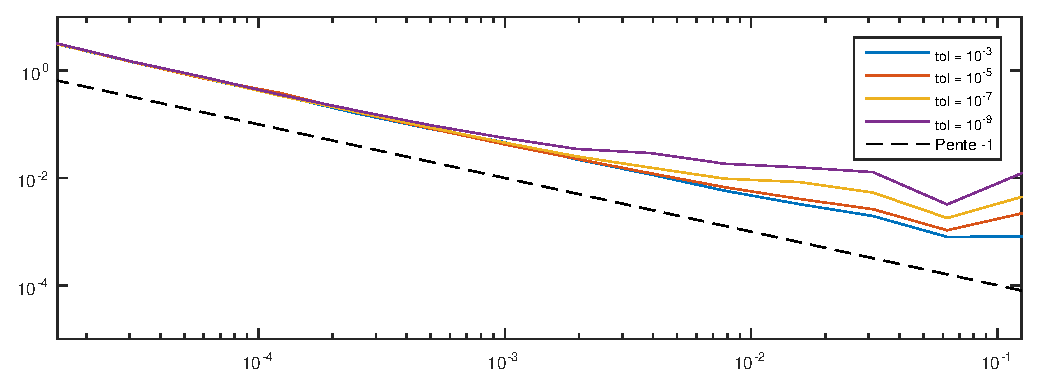
\includegraphics[width=.8\textwidth]{img/chap1/cost_rke.eps}
\caption{Temps de calcul (en s) avec notre méthode de Runge-Kutta imbriqués en fonction de $\epsilon$.}
\label{fig:cout_rke}
\end{figure}
\begin{figure}[!h]
\centering
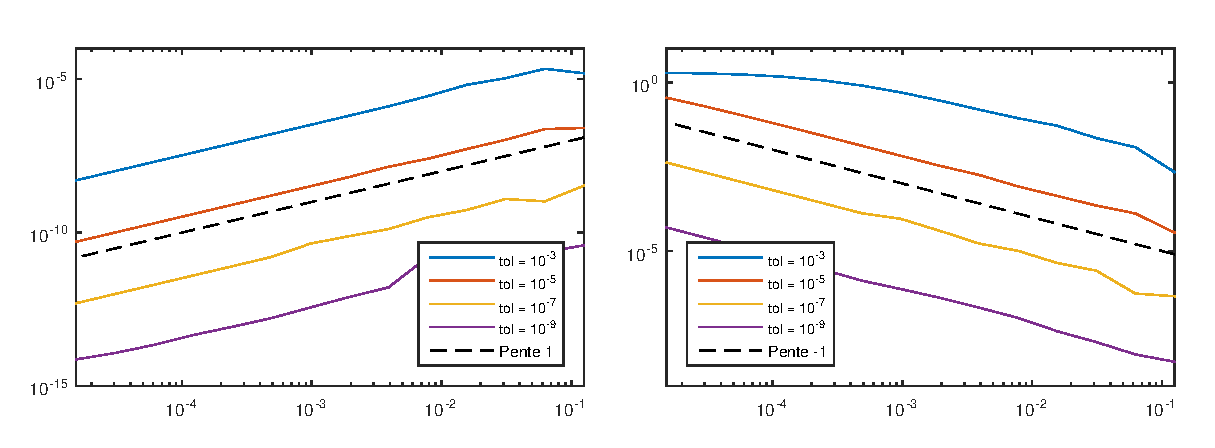
\includegraphics[width=\textwidth]{img/ann/conv_rel_rke.eps}
\caption{Erreur relative en norme absolue sur $x$ (à gauche) et sur $z$ (à droite) en fonction de $\epsilon$ pour le cas \eqref{pb:edo_partic_1} avec une méthode de Runge-Kutta imbriqués.}
\end{figure}

On voit alors que l'erreur sur $z$ augmente avec $\epsilon$ lorsque $\epsilon$ diminue, ce qui va à l'encontre de notre objectif. 
On rappelle en outre que le 

\section{Développement asymptotique}
\label{subsec:ann_asymp}

Dans \cite{castella2016formal}, on fournit les développement à l'ordre 3 en $\epsilon$ de la variété centrale $\epsilon h\eeps(\cdot)$ et de la condition initiale réduite $x_0\eeps$ dans les cas particuliers \eqref{pb:edo_partic_1} et \eqref{pb:edo_partic_2}. 
En particulier, dans le cas \eqref{pb:edo_partic_2}, on définit la variété tronquée et la condition initiale réduite tronquée 
\begin{align*}
\epsilon h^{[3]}(x) ={}& \epsilon x_1^2 x_2^2 - 2\epsilon^2 x_1 x_2(x_1^2 - x_2^2) + 2\epsilon^3 \left(x_1 x_2(x_1^2 - x_2^2 - 2) + (x_1^2 - x_2^2)^2 \right) \\
={}& \epsilon h\eeps(x) + \O(\epsilon^4), 
\end{align*}
\begin{multline*}
x_0^{[3]} = \left(1- \frac{\epsilon^2}{2}z_0^2 + \frac{\epsilon^3}{2} x_{0,1}^2 x_{0,2}^2 z_0 \right) x_0  
+ \Big[-\epsilon z_0 + \epsilon^2 x_{0,1}^2 x_{0,2}^2 \\
+ \epsilon^3 \left( \frac16 z_0^3 - 2(1+2 z_0)x_{0,1}x_{0,2}(x_{0,1}^2 - x_{0,2}^2) \right) \Big]
\begin{pmatrix} 0 & -1 \\ 1 & 0 \end{pmatrix} x_0 + = x_0\eeps + \O(\epsilon^4) .
%\qquad\qquad
\end{multline*} 

On définit la solution sur la variété approchée 
$$ \dot{x}^{[3]}_{\infty} = f(x^{[3]}_{\infty},\epsilon h^{[3]}\circ x^{[3]}_{\infty}), \qquad x^{[3]}_{\infty}(0) = x_0^{[3]} . $$
On peut alors la calculer et la comparer à la solution réelle en fonction du temps et on voit que l'écart diminue avec $\epsilon$. 
Vérifions que lors d'une simulation numérique, on obtient une erreur d'ordre $\O(\epsilon^4 + \dt^p)$ où $p$ est l'ordre de la méthode. 
L'erreur $\O(\epsilon^4)$ provient du modèle, de l'approximation de $x_0\eeps$ et $h\eeps$, tandis que l'erreur $\O(\dt^p)$ provient du calcul numérique de $x^{[3]}_{\infty}$. 

Pour la vérification, on commence par faire une résolution quasi-exacte sur la variété et sur le système initial pour vérifier la partie $\O(\epsilon^4)$, 
puis on fixe $\epsilon$ très faible et on résout le problème sur la variété approximée avec une méthode d'Euler explicite pour vérifier la partie $\O(\dt)$. 
Dans le cas \eqref{pb:edo_partic_1}, on a $\dot{x} = \O(\epsilon)$ sur la variété, donc cette approche est impossible 
(c'est pourquoi on utilise le cas \eqref{pb:edo_partic_2} pour ces tests). 

\begin{figure}[!h]
\centering
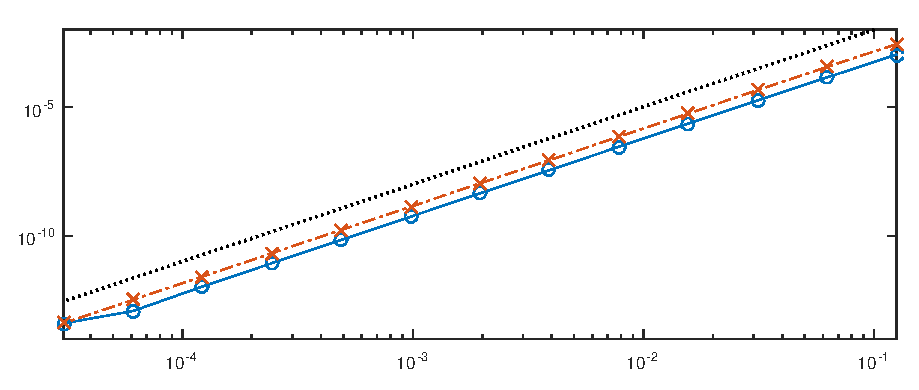
\includegraphics[width=.9\textwidth]{img/ann/erreur_manifold_approx.eps}
\caption{Différences entre $x\eeps$ et $x^{[3]}_{\infty}$ (ronds, trait plein bleu) et entre $z\eeps$ et $\epsilon h^{[3]}\circ x^{[3]}_{\infty}$ (croix, trait pointillé rouge) en fonction de $\epsilon$ en $t=1$, comparées à une pente $\epsilon^3$ (pointillés noirs) dans le cas test \eqref{pb:edo_partic_2}.}
\end{figure}
On voit alors que l'erreur est en $\O(\epsilon^3)$, ce qui n'est pas le résultat auquel on s'attendait. 
Il se peut que les formules de l'article soient erronées. 
En effet, en effectuant notre propre développement sur $h\eeps$ en remarquant $\dpz g = 0$, on obtient 
\begin{align*}
h\eeps(x) ={}& g(x,0) - \epsilon \dpx \left[ g(x,0) - \epsilon \dpx g(x,0)\cdot f(x,0) \right] \cdot f(x,\epsilon g(x,0)) + \O(\epsilon^3) \\
={}& g(x,0) - \epsilon \dpx g(x,0)\cdot f(x,0) + \epsilon^2 \dpx^2 g(x,0)\cdot (f(x,0),f(x,0)) 
\\ & + \epsilon^2 \dpx g(x,0)\cdot[ \dpx f(x,0)\cdot f(x,0) - \dpz f(x,0)\cdot g(x,0)] + \O(\epsilon^3) 
\end{align*} 
soit d'après nos calculs 
\begin{align*}
\epsilon h^{[3]}(x) ={}& \epsilon x_1^2x_2^2 - 2\epsilon^2 x_1x_2(x_1^2-x_2^2) + 2\epsilon^3 \left( x_1^2 x_2^2(x_1^3 x_2 - x_1 x_2^3 - 2) + (x_2^2-x_1^2)^2 \right). 
\end{align*}
Effectuer cette correction ne change pas les résultats, donc il se peut que la formule pour $x_0^{[3]}$ soit mal reportée dans l'article. 
On peut néanmoins vérifier la convergence en $\O(\dt)$ avec un schéma d'Euler explicite pour calculer la solution sur la variété approchée, dans le cas $\epsilon$ très petit (on choisit $\epsilon = 2^{-12}$). 
\begin{figure}[!h]
\centering
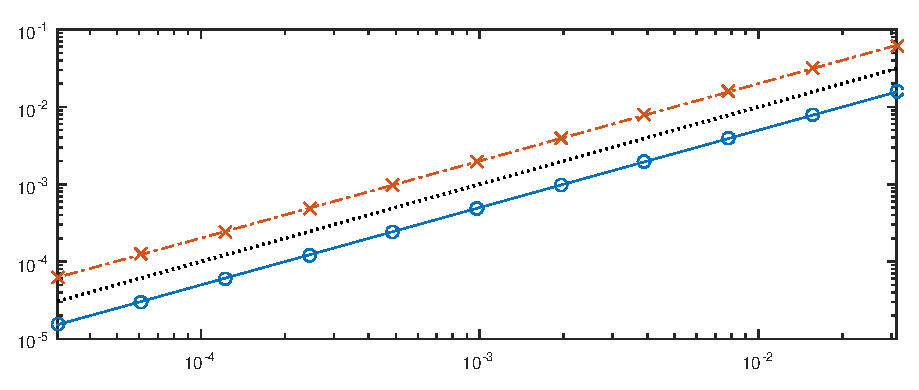
\includegraphics[width=.9\textwidth]{img/ann/erreur_manifold_euler.eps}
\caption{Différences entre $x\eeps$ et $x^{[3]}_{\infty}$ (ronds, trait plein bleu) et entre $z\eeps$ et $\epsilon h^{[3]}\circ x^{[3]}_{\infty}$ (croix, trait pointillé rouge) en fonction de $\dt$ en $t=1$ lorsque $x^{[3]}_{\infty}(1)$ est calculée par méthode d'Euler explicite de pas de temps $\dt$. La droite pointillée noire est de pente 1.}
\end{figure}

On voit alors que la convergence $\O(\dt)$ est bien vérifiée. 